\chapter{Johdanto}

Kurssin \emph{Tietorakenteet ja algoritmit} tarkoituksena
on opettaa menetelmiä, joiden avulla voimme ratkaista
\emph{tehokkaasti} laskennallisia ongelmia.
Ohjelmoinnin peruskursseilla olemme keskittyneet
ohjelmointitaidon opetteluun.
Nyt on aika siirtyä askel eteenpäin ja alkaa kiinnittää
huomiota myös siihen, miten tehokkaita ohjelmat ovat.

Algoritmien tehokkuudella on suuri merkitys käytännössä.
Esimerkiksi netissä toimiva reittiopas on käyttökelpoinen sen vuoksi,
että saamme reitin kuvauksen heti sen jälkeen kun olemme
ilmoittaneet, mistä mihin haluamme matkustaa.
Jos meidän pitäisi odottaa reitin kuvausta vaikkapa viikko tai kuukausi,
tämä rajoittaisi paljon palvelun käyttöä.

Jotta reittiopas toimisi tehokkaasti, sen taustalla on
hyvin suunniteltu algoritmi.
Tällä kurssilla opimme, kuinka voimme luoda itse vastaavia algoritmeja.
Tutustumme kurssilla sekä algoritmien suunnittelun teoriaan että
käytäntöön -- haluamme ymmärtää syvällisesti, mistä algoritmeissa on kysymys,
mutta myös osata toteuttaa niitä käytännössä.

\section{Laskennalliset ongelmat}

\emph{Laskennallinen ongelma} on hyvin määritelty laskentatehtävä,
jonka haluamme ratkaista.
Lähtökohtana on, että meille annetaan ongelman kuvaus,
jossa kerrotaan täsmällisesti algoritmille annettava
\emph{syöte} sekä haluttu \emph{tuloste}.
Syöte tarkoittaa, mitä tietoja algoritmille annetaan,
ja tuloste tarkoittaa, mitä algoritmin tulee tuottaa vastauksena.

Seuraavassa on esimerkki laskennallisesta ongelmasta:

\begin{itemize}
\item \textbf{Syöte}: Algoritmille annetaan taulukko,
jossa on $n$ kokonaislukua.
\item \textbf{Tuloste:} Algoritmin tulee ilmoittaa,
mikä on taulukon lukujen summa.
\end{itemize}

Esimerkiksi jos $n=4$ ja taulukko on $[2,1,5,2]$,
niin algoritmin tulee antaa vastaus $10$,
koska taulukon lukujen summa on $2+1+5+2=10$.

Voimme ratkaista tämän ongelman seuraavasti Javalla:

\begin{code}
int summa = 0;
for (int i = 0; i < n; i++) {
    summa += luvut[i];
}
System.out.println(summa);
\end{code}

Ensimmäinen vaihe ohjelmoinnin oppimisessa on oppia
ohjelmoinnin perustaidot niin, että osaamme kirjoittaa
jonkin toimivan koodin, joka ratkaisee annetun ongelman.
On arvokas taito sinänsä, että osaamme kirjoittaa
toimivan koodin ongelman ratkaisemiseen.
Toinen vaihe, johon keskitymme tällä kurssilla,
on oppia suunnittelemaan \emph{tehokkaita} algoritmeja.
Tämä tarkoittaa, että haluamme saada aikaan mahdollisuuksien mukaan
jotain parempaa kuin suoraviivaisia
raakaan voimaan perustuvia algoritmeja.

Kiehtova seikka ohjelmoinnissa on, että monimutkaisetkin algoritmit
syntyvät yksinkertaisista aineksista. Keskeiset käsitteet ovat

\begin{itemize}
\item muuttujat, joissa voimme säilyttää tietoa ohjelmassa,
\item ehtolause (\texttt{if}), jonka avulla voimme haarautua ohjelmassa,
\item silmukat (\texttt{for} ja \texttt{while}), joiden avulla voimme
toistaa laskentaa, sekä
\item taulukot, joissa voimme säilyttää paljon tietoa.
\end{itemize}

Itse asiassa voimme toteuttaa \emph{minkä tahansa} algoritmin
vain näitä aineksia käyttäen.
Tämä on huojentava tieto, koska meidän ei siis tarvitse opetella
suurta määrää ohjelmointikielten ominaisuuksia,
ennen kuin voimme alkaa suunnitella algoritmeja.
Vaikeutena on kuitenkin \emph{keksiä}, kuinka käyttää näitä
tekniikoita eri tilanteessa.

Käytämme kirjassa algoritmien esittämiseen Java-kieltä,
joka on tuttu ohjelmoinnin peruskursseilta,
ja käymme myös erikseen läpi Java-kielen
standardikirjaston tietorakenteita ja algoritmeja.
Ohjelmointikieli ei ole kuitenkaan merkittävässä osassa
algoritmien suunnittelussa, vaan kirjassa käsitellyt asiat
ovat voimassa myös muissa ohjelmointikielissä.

\section{Rekursiiviset algoritmit}

Ohjelmoinnin perusteiden opiskelussa rekursio jää usein sivurooliin,
mikä on vahinko, koska se on käytännössä hyödyllinen työkalu.
Voimme toteuttaa rekursion avulla kätevästi algoritmeja,
jotka käyvät järjestelmällisesti läpi ongelman ratkaisuja.
Seuraavaksi käymme läpi muutamia esimerkkejä siitä,
kuinka voimme hyödyntää rekursiota ohjelmoinnissa.

\subsection{Osajoukkojen läpikäynti}

Joukon osajoukkoja ovat kaikki tavat valita osa joukon alkioista.
Esimerkiksi joukon $\{1,2,3\}$ osajoukot ovat
$\emptyset$ (tyhjä joukko), $\{1\}$, $\{2\}$, $\{3\}$,
$\{1,2\}$, $\{1,3\}$, $\{2,3\}$ ja $\{1,2,3\}$.
Jos joukossa on $n$ alkioita, osajoukkoja on $2^n$.

Rekursio tarjoaa kätevän tavan käydä läpi kaikki
joukon osajoukot. Esimerkiksi seuraava koodi pitää yllä
rakennetta

\begin{code}
ArrayDeque<Integer> osajoukko;
\end{code}

joka sisältää vuorollaan kunkin joukon $\{1,2,\dots,n\}$
osajoukon.
Haku läh\-tee käyntiin, kun kutsumme metodia \texttt{muodosta}
parametrilla $1$.

\begin{code}
void muodosta(int x) {
    if (x == n+1) {
        System.out.println(osajoukko);
        return;
    }
    muodosta(x+1); // x ei valita osajoukkoon
    osajoukko.addLast(x);
    muodosta(x+1); // x valitaan osajoukkoon
    osajoukko.removeLast();
}
\end{code}

Jokaisessa kutsussa metodi käy läpi tapaukset,
otetaanko luku $x$ mukaan osajoukkoon vai ei.
Molemmissa tapauksissa metodi kutsuu itseään yhtä
suuremalla $x$:n arvolla.
Lopulta kun $x=n+1$, kaikki luvut on käyty läpi
ja on aika tulostaa osajoukko.

Esimerkiksi tapauksessa $n=3$ koodin tulostus on seuraava:

\begin{code}
[]
[3]
[2]
[2, 3]
[1]
[1, 3]
[1, 2]
[1, 2, 3]
\end{code}

\subsection{Permutaatioiden läpikäynti}

Joukon permutaatiot ovat kaikki tavat järjestää joukon alkiot.
Esimerkiksi joukon $\{1,2,3\}$ permutaatiot ovat
$(1,2,3)$, $(1,3,2)$, $(2,1,3)$, $(2,3,1)$, $(3,1,2)$ ja $(3,2,1)$.
Jos joukossa on $n$ alkiota, permutaatioita on $n!$.

Myös permutaatioiden läpikäynti onnistuu kätevästi rekursiolla.
Seuraava koodi pitää yllä rakennetta

\begin{code}
ArrayDeque<Integer> permutaatio;
\end{code}

joka sisältää vuorollaan kunkin joukon $\{1,2,\dots,n\}$ permutaation.
Haku lähtee käyntiin, kun kutsumme metodia
\texttt{muodosta} ilman parametreja.

\begin{code}
void muodosta() {
    if (permutaatio.size() == n) {
        System.out.println(permutaatio);
        return;
    }
    for (int i = 1; i <= n; i++) {
        if (!permutaatio.contains(i)) {
            permutaatio.addLast(i);
            muodosta();
            permutaatio.removeLast();
        }
    }
}
\end{code}

Tässä on ideana, että metodi käy joka kutsulla läpi kaikki luvut
$1,2,\dots,n$ ja aina jos luku ei kuulu vielä permutaatioon,
koodi haarautuu rekursiivisesti tapaukseen, jossa se lisätään
seuraavaksi permutaatioon.
Sitten kun permutaatiossa on $n$ lukua, se on valmis ja
voimme tulostaa sen.

Esimerkiksi tapauksessa $n=3$ koodin tulostus on seuraava:

\begin{code}
[1, 2, 3]
[1, 3, 2]
[2, 1, 3]
[2, 3, 1]
[3, 1, 2]
[3, 2, 1]
\end{code}

\subsection{Peruuttava haku}

\emph{Peruuttava haku} on yleinen rekursiivinen menetelmä,
jota käyttäen voimme muodostaa järjestelmällisesti
kaikki ratkaisut annettuun tehtävään.
Siinä on ideana aloittaa tyhjästä ratkaisusta ja käydä
joka askeleella läpi rekursiivisesti kaikki mahdolliset tavat laajentaa ratkaisua.

Peruuttava haku on raa'an voiman menetelmä,
ja voimme käyttää sitä vain silloin,
kun ratkaisujen määrä on niin pieni,
että ehdimme käydä kaikki läpi.
Kuitenkin jos voimme käyttää peruuttavaa hakua,
se on mainio tekniikka,
koska voimme olla varmoja, että oikein toteutettu
peruuttava haku löytää kaikki ratkaisut.

\begin{figure}
\center
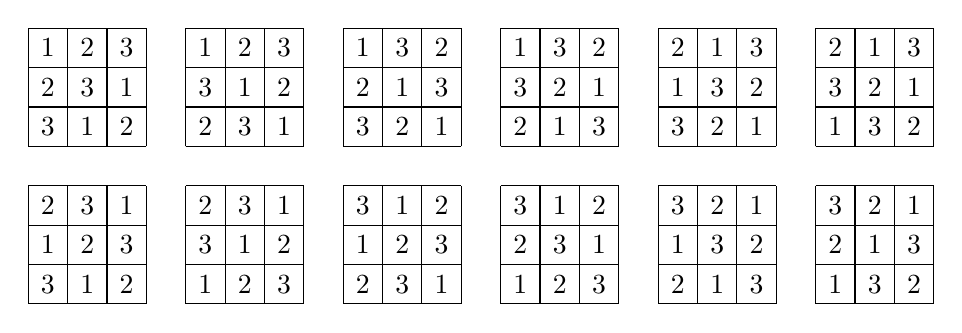
\begin{tikzpicture}[scale=0.5]
\newcommand\nelio[9]{
\draw (0,0) grid (3,3);
\foreach \x/\y/\v in {0/0/#1,1/0/#2,2/0/#3,0/1/#4,1/1/#5,2/1/#6,0/2/#7,1/2/#8,2/2/#9} \node at (0.5+\x,2.5-\y) {\v};
}
\begin{scope}
\nelio{1}{2}{3}{2}{3}{1}{3}{1}{2}
\end{scope}
\begin{scope}[xshift=4cm]
\nelio{1}{2}{3}{3}{1}{2}{2}{3}{1}
\end{scope}
\begin{scope}[xshift=8cm]
\nelio{1}{3}{2}{2}{1}{3}{3}{2}{1}
\end{scope}
\begin{scope}[xshift=12cm]
\nelio{1}{3}{2}{3}{2}{1}{2}{1}{3}
\end{scope}
\begin{scope}[xshift=16cm]
\nelio{2}{1}{3}{1}{3}{2}{3}{2}{1}
\end{scope}
\begin{scope}[xshift=20cm]
\nelio{2}{1}{3}{3}{2}{1}{1}{3}{2}
\end{scope}
\begin{scope}[yshift=-4cm]
\nelio{2}{3}{1}{1}{2}{3}{3}{1}{2}
\end{scope}
\begin{scope}[yshift=-4cm,xshift=4cm]
\nelio{2}{3}{1}{3}{1}{2}{1}{2}{3}
\end{scope}
\begin{scope}[yshift=-4cm,xshift=8cm]
\nelio{3}{1}{2}{1}{2}{3}{2}{3}{1}
\end{scope}
\begin{scope}[yshift=-4cm,xshift=12cm]
\nelio{3}{1}{2}{2}{3}{1}{1}{2}{3}
\end{scope}
\begin{scope}[yshift=-4cm,xshift=16cm]
\nelio{3}{2}{1}{1}{3}{2}{2}{1}{3}
\end{scope}
\begin{scope}[yshift=-4cm,xshift=20cm]
\nelio{3}{2}{1}{2}{1}{3}{1}{3}{2}
\end{scope}
\end{tikzpicture}
\caption{Kaikki 12 latinalaista neliötä kokoa $3 \times 3$.}
\label{fig:latnel}
\end{figure}

Tarkastelemme esimerkkinä tehtävää, jossa haluamme laskea,
montako $n \times n$ -kokoista latinalaista neliötä on olemassa.
\emph{Latinalainen neliö} on ruudukko, jonka
kullakin vaaka- ja pystyrivillä esiintyy tarkalleen kerran
jokainen luku $1,2,\dots,n$.
Kyseessä on siis yksinkertaisempi muoto tutusta sudoku-tehtävästä.
Esimerkiksi kuvassa \ref{fig:latnel} on kaikki 12 latinalaista neliötä kokoa $3 \times 3$.
Kun $n$ kasvaa, niin ratkaisujen määrä kasvaa nopeasti.

Hakua varten määrittelemme seuraavat taulukot:

\begin{code}
int[][] nelio = new int[n][n];
boolean[][] vaaka = new boolean[n][n];
boolean[][] pysty = new boolean[n][n];
\end{code}

Numeroimme ruudukon pysty- ja vaakarivit $0,1,\dots,n-1$.
Tarkoituksena on, että kohdassa $\texttt{nelio}[y][x]$
on neliössä ruudussa $(y,x)$ oleva luku.
Lisäksi $\texttt{vaaka}[y][k]$ kertoo, onko vaakarivillä $y$
jo lukua $k$, ja vastaavasti $\texttt{pysty}[x][k]$ kertoo,
onko pystyrivillä $x$ jo lukua $k$.
Alussa kaikki taulukot ovat tyhjiä ja täytämme niitä
pikkuhiljaa peruuttavan haun aikana.

Seuraava rekursiivinen metodi toteuttaa haun, kun sille
annetaan alkuparametreina $y=0$ ja $x=0$.
Metodi laskee latinalaisten neliöiden määrän muuttujaan 
\texttt{laskuri}.

\begin{code}
static void muodosta(int y, int x) {
    if (y == n) laskuri++;
    else if (x == n) muodosta(y+1,0);
    else {
        for (int i = 1; i <= n; i++) {
            if (!vaaka[y][i] && !pysty[x][i]) {
                vaaka[y][i] = pysty[x][i] = true;
                nelio[y][x] = i;
                muodosta(y, x+1);
                vaaka[y][i] = pysty[x][i] = false;
            }
        }
    }
}
\end{code}

Jokaisella askeleella metodi valitsee luvun ruutuun
$(y,x)$ ja siirtyy seuraavaan ruutuun oikealle.
Jos $x=n$, vaakarivi on tullut täyteen ja metodi siirtyy
seuraavalle vaakariville.
Jos taas $y=n$, koko ruudukko on tullut täyteen ja
metodi kasvattaa ruudukoiden määrää yhdellä.

\begin{table}
\center
\begin{tabular}{rr}
ruudukon koko $n$ & neliöiden määrä \\
\hline
1 & 1 \\
2 & 2 \\
3 & 12 \\
4 & 576 \\
5 & 161280 \\
6 & 812851200 \\
\end{tabular}
\caption{Latinalaisten neliöiden määriä pienille $n$:n arvoille.}
\label{tab:latnel}
\end{table}

Tämän koodin avulla voimme laskea latinalaisten neliöiden
määrät ensimmäisille $n$:n arvoille.
Taulukko \ref{tab:latnel} näyttää nämä tulokset.
Suuremmilla $n$:n arvoilla haku alkaa kestää liian kauan
ja meidän tulisi keksiä keino tehostaa hakua,
jos haluaisimme laskea tuloksia suuremmille arvoille.

\section{Matemaattinen tausta}

Tietorakenteiden ja algoritmien teoria perustuu matematiikkaan,
ja käym\-me kirjassa pikkuhiljaa läpi tarvittavia tietoja.
Seuraavassa on joitakin merkintöjä ja käsitteitä, joista on hyötyä
useassa kirjan kohdassa.

\subsection{Summakaavat}

Voimme laskea lukujen $1,2,\dots,n$ summan kaavalla
\[1+2+\dots+n = \frac{n(n+1)}{2}.\]
Esimerkiksi
\[1+2+3+4+5 = \frac{5 \cdot 6}{2}=15.\]
Kaavan voi ymmärtää niin, että laskemme yhteen $n$ lukua,
joiden suuruus on \emph{keskimäärin} $(n+1)/2$.

Toinen hyödyllinen kaava on
\[2^0+2^1+\dots+2^n = 2^{n+1}-1.\]
Esimerkiksi
\[1+2+4+8+16=32-1.\]
Tässä voimme ajatella, että aloitamme luvusta $2^n$
ja lisäämme siihen aina puolet pienemmän luvun lukuun $1$ asti.
Tämän seurauksena pääsemme yhtä vaille lukuun $2^{n+1}$ asti.

Esitämme joskus summia merkinnän $\sum$ avulla.
Siinä on ideana antaa muuttujan ala- ja yläraja sekä
joka askeleella summaan lisättävä arvo.
Esimerkiksi voimme merkitä
\[1^2 + 2^2 + \dots + n^2 = \sum_{i=1}^n i^2.\]

Tämä merkintä on itse asiassa hyvin lähellä ohjelmoinnin
for-silmukkaa, koska seuraava koodi ajaa saman asian:

\begin{code}
int summa = 0;
for (int i = 1; i <= n; i++) {
    summa += i*i;
}
\end{code}

\subsection{Logaritmit}

Logaritmin määritelmän mukaan $\log_b(n)=a$
tarkalleen silloin kun $b^a=n$.
Esimerkiksi $\log_2(32)=5$, koska $2^5=32$.

Algoritmiikassa logaritmin kantaluku $b$ on usein 2,
ja voimme ajatella, että logaritmi kertoo, montako kertaa
meidän tulee puolittaa luku $n$, ennen kuin pääsemme lukuun 1.
Esimerkiksi $\log_2(32)=5$, koska tarvitsemme 5 puolitusta:
\[32 \rightarrow 16 \rightarrow 8 \rightarrow 4 \rightarrow 2 \rightarrow 1\]

Logaritmeille pätee kaavat
\[\log_b(x \cdot y) = \log_b(x)+\log_b(y)\]
ja
\[\log_b(x / y) = \log_b(x)-\log_b(y).\]
Ylemmästä kaavasta seuraa myös
\[\log_b(x^k) = k \log_b(x).\]
Lisäksi voimme vaihtaa logaritmin kantalukua kaavalla
\[\log_u(x) = \frac{\log_b(x)}{\log_b(u)}.\]